\documentclass{article}

\usepackage[final]{style}
\usepackage[utf8]{inputenc} % allow utf-8 input
\usepackage[T1]{fontenc}    % use 8-bit T1 fonts
\usepackage{hyperref}       % hyperlinks
\usepackage{url}            % simple URL typesetting
\usepackage{booktabs}       % professional-quality tables
\usepackage{amsfonts}       % blackboard math symbols
\usepackage{nicefrac}       % compact symbols for 1/2, etc.
\usepackage{microtype}      % microtypography
\usepackage{verbatim}
\usepackage{graphicx}       % for figures

\title{Lecture \#7: Model-Based Reinforcement Learning, Advanced Model Learning and Images}

\author{
  Lee Yong Ler, Lin Qian \\
  Department of Computer Science\\
  National University of Singapore\\
  Singapore, S117417 \\
}

\begin{document}

\maketitle


\section{Introduction}
In reinforcement learning RL, we maximize the rewards for our actions. By simply looking at the equation below, rewards depend on the policy and the system dynamics (model).

Model-based reinforcement learning requires less samples and allow the agent to plan by thinking ahead. However, it involves complex optimization methods and more assumptions and approximations.

\section{Summary of Model-free RL vs Model-based RL}

\begin{figure}[h]
    \centering
        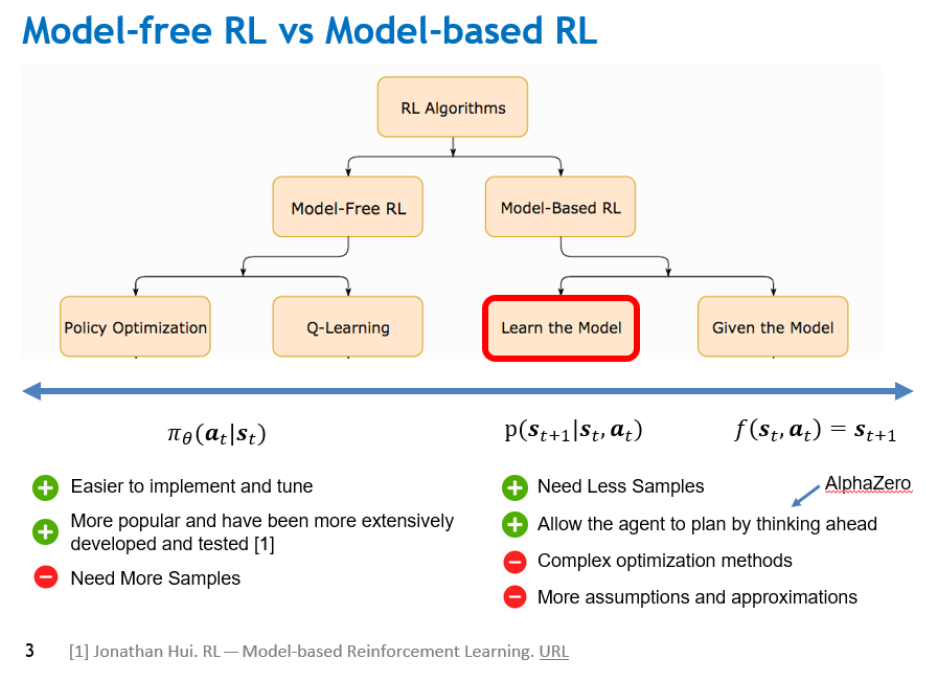
\includegraphics[width=0.8\linewidth]{img/vs.png}
    \caption{Overview: Model-free RL vs Model-based RL}
    \label{fig:vs}
\end{figure}

\noindent\textbf{DAgger} First you collect data with initial policy then you get more data then you obtain another initial policy.
\begin{itemize}
\item[--] To try to mitigate the variation when you do not follow the same trajectory
\end{itemize}

\noindent\textbf{Version 1.5} Instead of doing all actions, we execute the first action and observe the resulting state and re-plan.
\begin{itemize}
\item[--] Planning not cheap
\end{itemize}

\noindent\textbf{Version 2.0}

\begin{figure}[h]
    \centering
        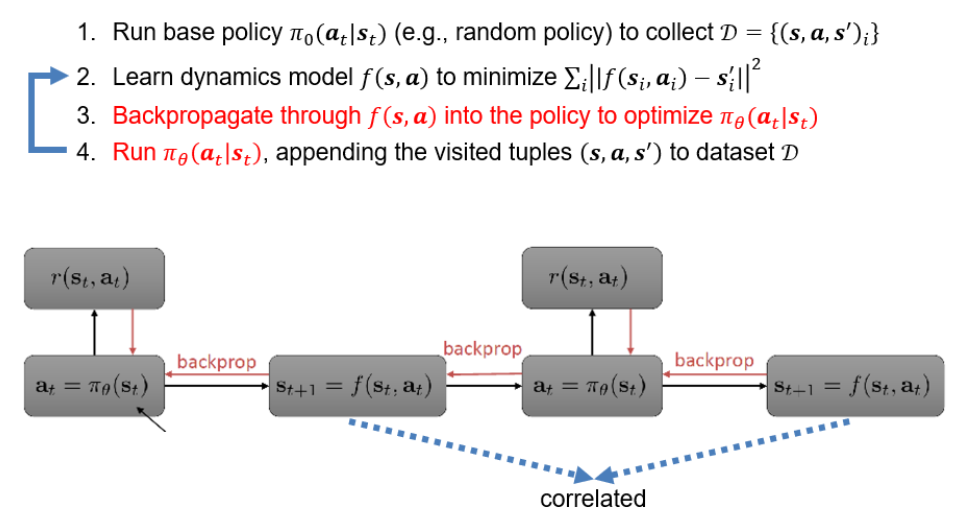
\includegraphics[width=0.8\linewidth]{img/v2.png}
    \caption{Version 2.0   Typo in image, $a_{t+1}$ at the third step instead of $a_{t}$ in between correlated states}
    \label{fig:v2}
\end{figure}

Backpropagate to optimize
\begin{itemize}
\item[--] Face exploding or vanishing gradient problem due to correlation
\end{itemize}

\section{System Dynamics representation models}
\subsection{Gaussian (\char`\~ Model-based 2.0)}
Gaussian: learn Gaussian Process model probability $p(s’|s,a)$ to maximize the sum of probability
\begin{itemize}
\item[--] Perform BP on probability to optimize the policy
\item[--] Performance: data-efficient, not great with non-smooth dynamics
\end{itemize}

\subsection{Neural Network}
Input: current status and action\\
Output: next status\\
Euclidean training loss (complex) corresponds to Gaussian probability $p(s’|s,a)$\\
Performance: Very expressive (data-consuming), not great when data size is small
\subsection{Gaussian Mixture Model}

\subsection{Problem with global models}
\begin{itemize}
\item[--] Big neural network or GP
\item[--] Planner will go to places where model erroneously thinks things are better than what	they really are
\item[--] Generally hard to find a good model converge to an accurate policy in most of the state space
\item[--] he model could be too complex comparing with policy
\end{itemize}

\subsection{Local models}
\begin{figure}[htp]
    \centering
        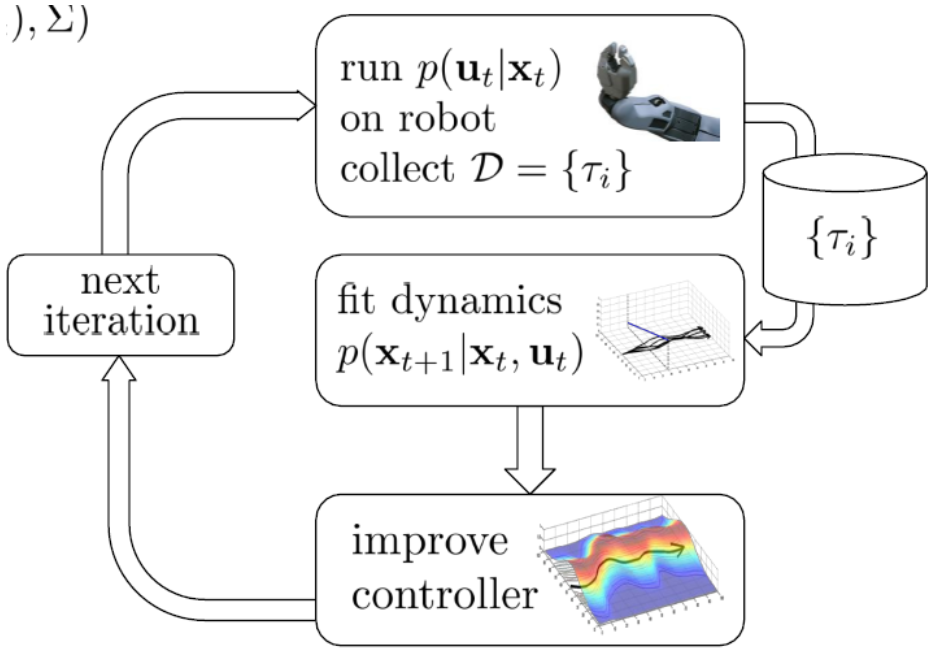
\includegraphics[width=0.5\linewidth]{img/localmodels.png}
    \caption{Overview: Local models}
    \label{fig:localmod}
\end{figure}
\textbf{Q: Why do we add a Gaussian noise?}\\
\begin{itemize}
\item[--] If deterministic, you won’t be able to find a correlation of current state with your next state. With noise you would be able to find a link between the current state and the next state.
\item[--] Without noise, all of the state would be at the same point. With noise, you would be able to do a linear regression on the same point. (can get a piecewise linear approximation of the function)
\item[--] Will be able to see more next state.
\end{itemize}
\textbf{Problem}
\begin{itemize}
\item[--] What controller to execute
\item[--] How to stay close to old controller
\end{itemize}

\subsection{Version 2.0 Controller}
\begin{figure}[htp]
    \centering
        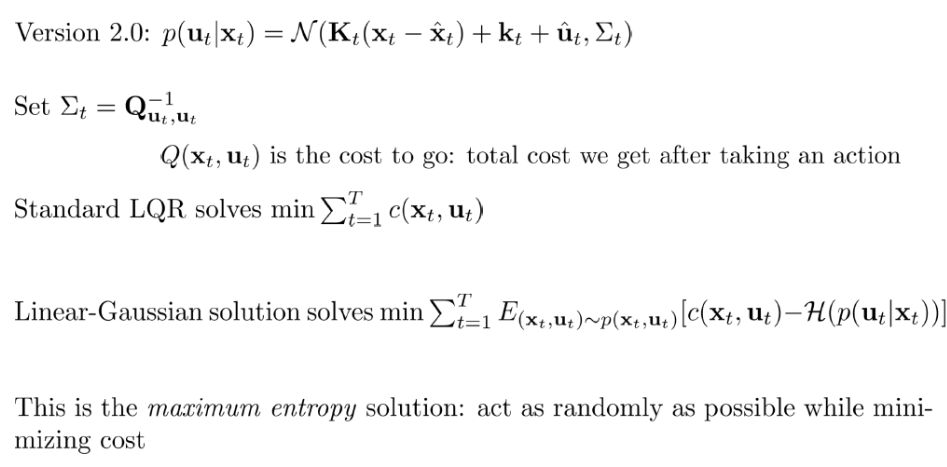
\includegraphics[width=0.8\linewidth]{img/v2control.png}
    \label{fig:v2control}
\end{figure}
Injecting more noise when the action is not that important, less when it matters.\\\\
\textbf{Q: Are we adding noise to two places, in the transition and the policy?}
\begin{itemize}
\item[--] Yes. Transition noise is to help to you get whether this action matters.
\end{itemize}
\begin{figure}[htp]
    \centering
        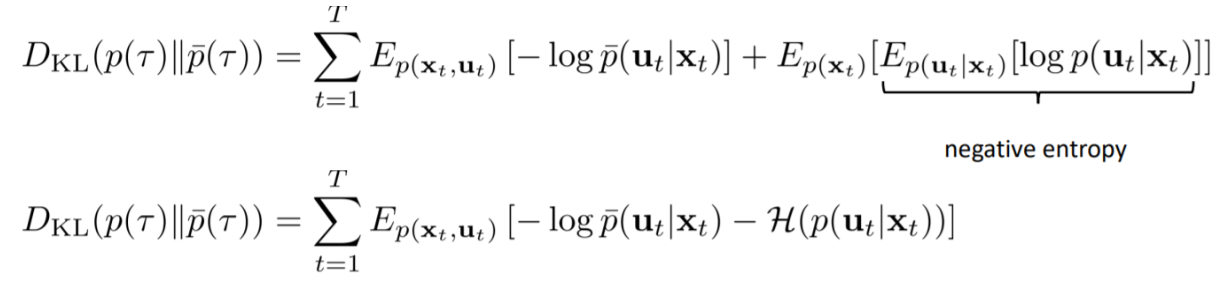
\includegraphics[width=0.8\linewidth]{img/dkl.png}
    \label{fig:dkl}
\end{figure}
\begin{itemize}
\item[--] Expectation under $x(t)$ of the expectation under $u(t)|x(t)$ is the same
\item[--]Expectation under $x(t)$ with probability theory
\end{itemize}

\begin{figure}[h]
    \centering
        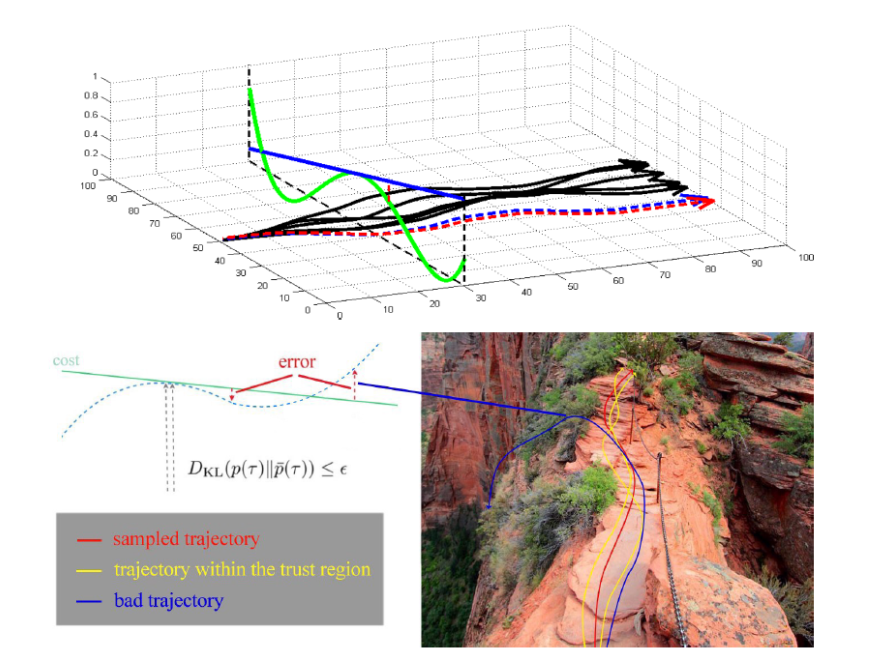
\includegraphics[width=1\linewidth]{img/traj.png}
    \caption{If we stray too far from old controller, may veer too far from the trajectory.}
    \label{fig:traj}
\end{figure}

\subsection{How to stay close to old controller}
Use KL divergence to find trust region
\begin{figure}[h]
    \centering
        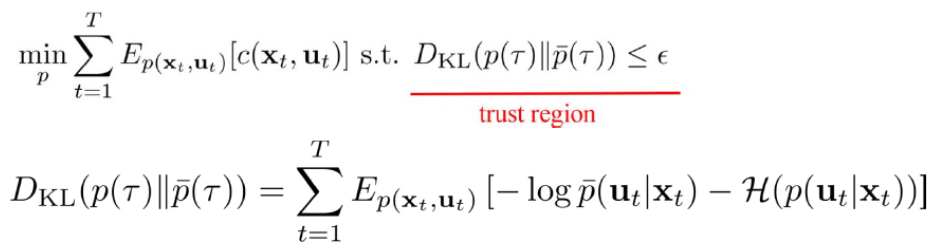
\includegraphics[width=0.8\linewidth]{img/trust.png}
    \label{fig:trust}
\end{figure}

Dual Gradient Descent
\begin{itemize}
\item[--] Transform the objective into a Lagrange dual function which can be optimized iteratively.
\end{itemize}
\begin{figure}[h]
    \centering
        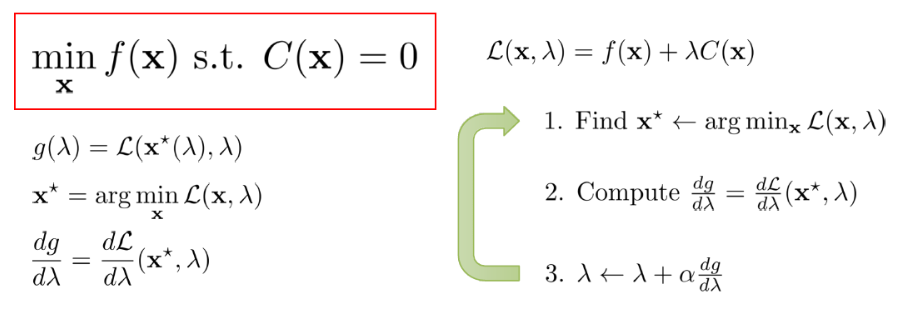
\includegraphics[width=0.8\linewidth]{img/dualgrad.png}
    \caption{Dual gradient descent}
    \label{fig:dgrad}
\end{figure}

\section{Managing overfitting in model-based RL}
Problem: Performance gap (pure model-based vs model-free)
Example: model based RL version 1.5
\begin{itemize}
\item[--] Trapped by a sudden increasing on reward
\end{itemize}
\begin{figure}[h]
    \centering
        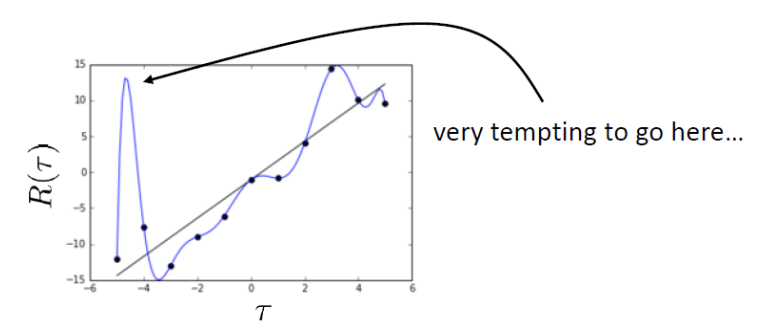
\includegraphics[width=0.7\linewidth]{img/tp.png}
    \label{fig:tp}
\end{figure}
\textbf{How to get uncertainty-aware model?}
\begin{enumerate}
   \item Use output entropy from a NN which output probability of next state given the current state and action
    \begin{enumerate}
     \item Will try to fit noise with data generation but there is still uncertainty cos of your model (there are two type of uncertainty statistical uncertainty and model uncertainty)
    \end{enumerate}
    \item Estimation of $p(\theta|D)$ where $\theta$ are the parameters
\end{enumerate}

\textbf{Bootstrap Ensemble}
\begin{itemize}
\item[--] Averaging of different network trained on a dataset made with sample with replacement
\item[--] Normal bootstrap used in machine learning
\item[--] In practice do not need resampling cos initialization of NN makes models independent anyway
\end{itemize}

\textbf{Q: How does dropout differ from bootstrapping ?}
\begin{itemize}
\item[--] Variance from different model low, we can trust the models but if variance really high, we would not trust any of the model. Drop out would not allow us to know the variance.
\end{itemize}

\textbf{Algorithm to evaluate models} (Figure \ref{fig:al2})\\
Run step 1-3 in $k$ neural network and average at step 4 so that you will know how good this action sequence is.
\begin{figure}[tbh]
    \centering
        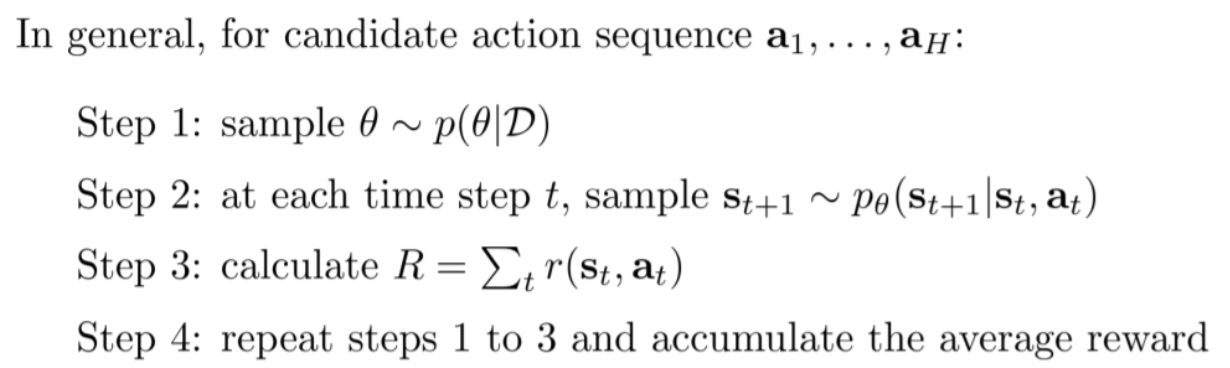
\includegraphics[width=0.7\linewidth]{img/al2.png}
    \caption{Evaluation steps}
    \label{fig:al2}
\end{figure}

\section{Usage of images in Model-based RL (Learning latent space)}
\begin{enumerate}
   \item Use bottleneck of autoencoder and feed into policy to output action
   \item Learning embedding then learn latent space
   \item Learning both embedding and image together (learning interested version of image only)
   \item Directly learning the next observation using another model
\end{enumerate}

\textbf{Q: What is spatial \textit{softmax}?}
\begin{itemize}
\item[--] \textit{Softmax} across the different channels
\item[--] Tensorflow definition compute the \textit{softmax} for each channel, get three pairs of (x, y), location of them.
\end{itemize}

% References
\small
\bibliographystyle{plain}
\bibliography{bibliography}
\end{document}
